\chapter{Testowanie zabezpieczeń IoT}
\label{chap:rozdzial5}
\section{Przeprowadzenie testów zabezpieczeń w środowisku testowym}
\subsection{Metodologia testów zabezpieczeń w środowisku testowym}
Proces testowy w każdym scenariuszu obejmował: 
\begin{enumerate}
    \item \textbf{Fazę przygotowawczą}, w której skonfigurowano środowisko testowe, ustalono metryki bazowe (baseline) dla wydajności systemu oraz zweryfikowano poprawność działania wszystkich komponentów.
    \item \textbf{Fazę wykonawczą}, w której przeprowadzano zaplanowany scenariusz ataku, równolegle monitorując parametry systemu oraz yellowdokumentując wszystkie obserwacje.
    \item \textbf{Fazę analityczną}, w której przeanalizowano zebrane dane, zweryfikowano skuteczność zabezpieczeń oraz zidentyfikowano potencjalne luki.
\end{enumerate}

\subsubsection{ARP Spoofing przy użyciu Bettercap}
Celem ataku ARP Spoofing było przejęcie kontroli nad komunikacją między urządzeniem IoT (Raspberry Pi oraz poidła dla psa Xiaomi) a routerem w sieci lokalnej. Atak umożliwił przekierowanie ruchu sieciowego przez urządzenie atakującego, co stanowiło podstawę do późniejszego zbadania podatności urządzeń IoT na ataki typu Man-in-the-Middle (MITM).
Narzędzie Bettercap zostało uruchomione w trybie interaktywnym z uprawnieniami administratora: \textit{sudo bettercap -iface eth0}, gdzie eth0 to interfejs atakującego. Przed rozpoczęciem ataku przeprowadzano pasywne skanowanie sieci w celu identyfikacji aktywnych hostów: \textit{net.probe on} oraz \textit{net.show}. Wynikiem było wykrycie: Raspberry Pi (192.168.1.39), urządzenia Xiaomi (192.168.1.25) oraz serwera MQTT (192.168.1.45). Wynik tego skanowania prezentuje Rysunek \ref{fig:Wyświetlenie listy urządzeń, przy użyciu Bettercap}.
\begin{figure}[h]
    \centering
    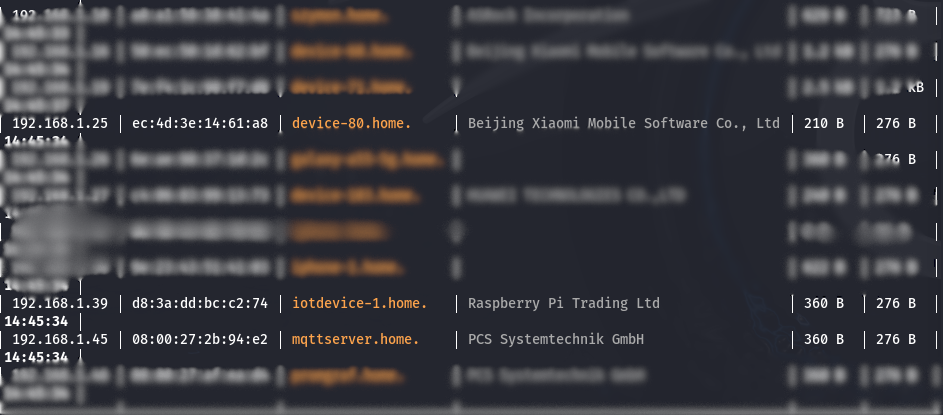
\includegraphics[width=0.8\textwidth]{pictures/net-show.png}
    \caption{Wyświetlenie listy urządzeń, przy użyciu Bettercap}
    \label{fig:Wyświetlenie listy urządzeń, przy użyciu Bettercap}
\end{figure}

W obu przypadkach atak polegał na wysyłaniu fałszywych odpowiedzi ARP, aby przekierować ruch ofiary przez system atakującego: \textit{set arp.spoof.targets 192.168.1.25 192.168.1.39}. W efekcie Kali Linux stał się pośrednikiem między urządzeniami a Routerem, wszystkie pakiety przesyłane przez ofiarę były przekierowywane.

\subsubsection{Sniffing ruchu sieciowego}
Po skutecznym przeprowadzeniu ataku ARP Spoofing, w którym ruch pomiędzy urządzeniami IoT (Raspberry Pi, poidło Xiaomi) a routerem został przekierowany przez system atakującego (Kali Linux), przystąpiono do przechwytywania i analizy danych. Wykorzystano narzędzia pasywne i aktywne w celu zbadania zawartości początkowo nieszyfrowanych komunikatów przesyłanych protokołami MQTT. 
W pierwszym etapie, za pomocą Wiresharka przechwycono nieszyfrowane komunikaty MQTT, identyfikując m.in dane przesyłane do brokera MQTT. Potwierdzono wyciek danych oraz niską odporność na wyciek danych.
Po pierwszej próbie, wdrożono zabezpieczenia przy użyciu protokołu TLS, po czym ponownie wykonano całą procedurę.

\subsubsection{Brute-force haseł}
Głównym celem przeprowadzonych testów była ocena skuteczności mechanizmów ochronnych urządzeń IoT oraz infrastruktury z nią bezpośrednio powiązanej, przed zautomatyzowanymi atakami słownikowymi. Badania obejmowały: analizę podatności na ataki brute force oraz weryfikację reakcji systemowych na wielokrotne próby logowania.
Testy przeprowadzono w kontrolowanym środowisku laboratoryjnym, z przygotowaną wcześniej infrastrukturą testową, w której aktywowano usługę SSH oraz MQTT z uwierzytelnieniem, tworząc przy tym testowe konto ze słabym hasłem. Następnie przygotowano dużą bazę haseł w formacie \textit{.txt}.
Najpierw przeprowadzono atak na protokół SSH, wykorzystując narzędzie Hydra i polecenia: \textit{hydra -l szymo -P passwordlist.txt 192.168.1.40 ssh -t 4 -vV -I}. Następnie przeprowadzano atak brute-force na broker MQTT. 

\subsubsection{Ataki DDoS}
W ramach badań przeprowadzono serię kontrolowanych ataków na środowisko testowe, w którym wyłączone zostały dodatkowe, nieistotne usługi w celu eliminacji zakłóceń. 
W pierwszym przypadku przeprowadzono atak na niezabezpieczony protokołem TLS broker MQTT, który nie wymagał uwierzytelnienia. Przy użyciu biblioteki \textit{paho.mqtt.client}, która jest bezpośrednią biblioteką do komunikacji z brokerem MQTT, stworzono skrypt w Pythonie.
\begin{lstlisting}[caption=Skrypt w Pythonie, label=lst:sensor]
    import paho.mqtt.client as mqtt
    import time
    
    broker = "192.168.1.45"
    port = 1883
    
    def flood_mqtt():
        while True:
            client = mqtt.Client()
            client.connect(broker, port)
            client.publish("test/flood", "Atak DDoS" * 1000)
            time.sleep(0.1)
    
    flood_mqtt()
\end{lstlisting}
W skrypcie przypisano adres IP brokera MQTT oraz port, na którym działa. Następnie w funkcji \textit{flood\_mqtt()} utworzono pętlę, która łączy się z brokerem i wysyła wiadomości na temat \textit{test/flood} co 0.1 sekundy. W ten sposób generowano dużą ilość ruchu, co prowadziło do przeciążenia brokera.
Podczas badania monitorowano parametry systemowe brokera MQTT.

W następnym przypadku przeprowadzono atak DDoS i DoS na protokół MQTT. Kluczowym elementem było użycie narzędzia hping3, a dokładnie polecenia: \textit{hping3 -S --flood -p 1883 192.168.1.45} w przypadku ataku z jednego adresu IP źródłowego oraz ataku rozproszonego, czyli przez zastosowanie \textit{--rand-source}. Jest to atak typu SYN Flood na port 1883 (port MQTT), wykorzystujący mechanizm nawiązywania połączeń TCP (tzw. three-way-handshake). Atakujący wysyła masowo pakiety SYN (żąda połączenia), serwer odpowiada pakietem SYN-ACK i rezerwuje zasoby (oczekuje ACK), natomiast atakujący nie wysyła ACK i pozostawia połączenie w stanie pół-otwartym.

Następnie przeprowadzono w identyczny sposób atak na protokoły UDP/55, UDP/123, TCP/22.

Na końcu przygotowano stronę HTTP, aby poddać ją ataku, przy użyciu narzędzia GoldenEye. Jest to narzędzie do przeprowadzania ataków DDoS warstwy aplikacji (HTTP Flood), które przeciąża cel poprzez masowe wysyłanie żądań HTTP. Jest napisane w Pythonie i działa na zasadzie generowania wielu równoległych połączeń, symulując ruch od wielu użytkowników. Wykonano polecenie \textit{python3 goldeneye.py http://192.168.1.45}, które: wysyła ogromną liczbę żądań HTTP (GET/POST), utrzymuje otwarte połączenia oraz używa losowych ścieżek URL. Narzędzie działa wielowątkowo, co pozwala na efektywne wykorzystanie zasobów atakującego. Wynik przechwycenia pakietów podczas tego ataku za pomocą narzędzia Wireshark przedstawia Rysunek \ref{fig:Przechwycone pakiety z programu Wireshark podczas ataku GoldenEye}.
\begin{figure}[h]
    \centering
    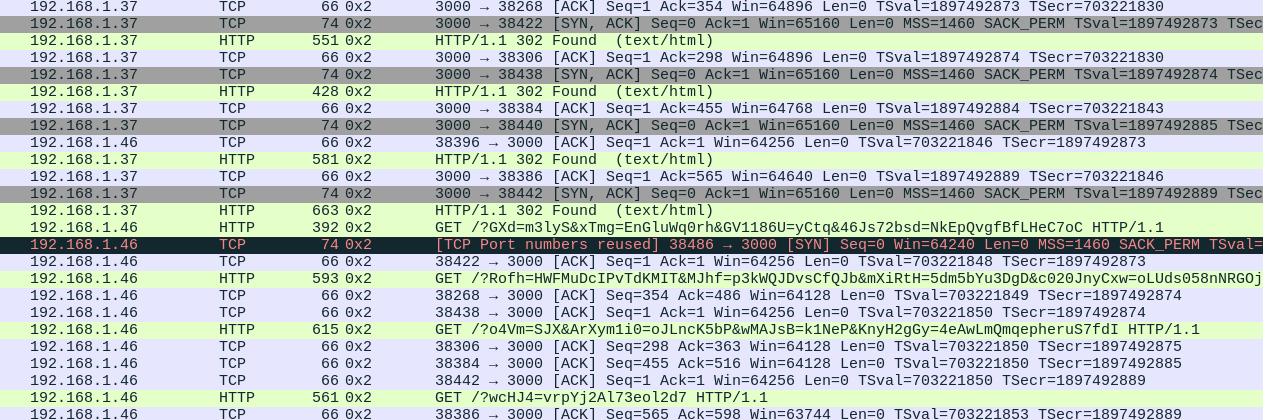
\includegraphics[width=0.8\textwidth]{pictures/wireshark-goldeneye.png}
    \caption{Przechwycone pakiety z programu Wireshark podczas ataku GoldenEye}
    \label{fig:Przechwycone pakiety z programu Wireshark podczas ataku GoldenEye}
\end{figure}

\subsection{Narzędzia wykorzystywane do testowania}
Narzędzia, które zostały wykorzystane w każdym scenariuszu i pozostawały niezmienne to:
\begin{itemize}
    \item \textbf{Infrastruktury sieciowej}: Router Wi-Fi, switch
    \item \textbf{System monitorujący:} Prometheus + Grafana na serwerze Ubuntu
\end{itemize}

\subsubsection{ARP Spoofing przy użyciu Bettercap}
Testy przeprowadzono w kontrolowanym środowisku laboratoryjnym, składającym się z:
\begin{itemize}
    \item \textbf{Urządzenia IoT:} Raspberry Pi 4B, pełniącego rolę urządzenia IoT, Xiaomi Pet Fountain
    \item \textbf{Stanowiska atakującego: } Laptop z Kali Linux (narzędzia: Bettercap, Metasploit, Wireshark, Nmap) 
\end{itemize}

\subsubsection{Sniffing ruchu sieciowego}
Testy przeprowadzono w prawie tym samym środowisku laboratoryjnym, co opisano w poprzednim scenariuszu (wykorzystując m.in. Raspberry Pi 4B oraz infrastrukturę sieciową). Do przechwycenia i analizy danych użyto narzędzi dostępnych na stanowisku atakującego (Kali Linux), w szczególności:
\begin{itemize}
    \item \textbf{Bettercap} - główna platforma do przeprowadzenia ataku ARP Spoofing oraz pasywnego sniffingu ruchu (moduły \textit{arp.spoof}, \textit{net.sniff}).
    \item \textbf{Wireshark} - narzędzie do analizy przechwyconych pakietów, umożliwiające wizualizację i dekodowanie różnych protokołów MQTT.
    \item \textbf{Nmap} - Dodatkowe skanowanie portów w celu weryfikacji aktywnych usług na urządzeniu IoT.
\end{itemize}

\subsubsection{Brute-force haseł}
Testy bezpieczeństwa przeprowadzono zgodnie z podejściem etycznego hakowania (ethical hacking), z wykorzystaniem następujących narzędzi:
\begin{itemize}
    \item \textbf{Urządzenia docelowe} - Raspberry Pi 4B, działające jako urządzenie IoT oraz Broker MQTT
    \item \textbf{Stacja atakująca} - Kali linux z narzędziami: Hydra, mqtt-pwn.
    \item \textbf{Słownik haseł} - Plik tekstowy z hasłami, zawierający 1000000 popularnych haseł, w tym domyślne hasła dla SSH i MQTT. 
\end{itemize}

\subsubsection{Ataki DDoS}
Testy przeprowadzono w kontrolowanym środowisku laboratoryjnym, składającym się z:
\begin{itemize}
    \item \textbf{Urządzenia docelowego} - Raspberry Pi 4 oraz broker MQTT Mosquitto.
    \item \textbf{Komputera atakującego} - Kali Linux z zainstalowanym Hping3, GoldenEye.
    \item \textbf{Python} - Język programowania.
    \item \textbf{Paho MQTT, time} - Biblioteka do komunikacji z brokerem MQTT, wykorzystywana do przeprowadzania ataków DoS.
\end{itemize}

\section{Ocena skuteczności zabezpieczeń IoT}
\subsection{Odporność na próby ataków}
\subsubsection{ARP Spoofing przy użyciu Bettercap}
Atak ARP spoofing został przeprowadzony w celu przejęcia kontroli nad komunikacją pomiędzy urządzeniem Xiaomi a routerem w sieci lokalnej. Urządzenie Xiaomi nie wykryło manipulacji w tablicy ARP, co potwierdziło brak mechanizmów obronnych na poziomie warstwy drugiej (L2). W urządzeniu nie zaimplementowano metod weryfikacji spójności tablic ARP, takich jak Secure ARP (S-ARP).

W kolejnym etapie badań przeprowadzono atak typu Man-in-the-Middle (MITM) na urządzenie Raspberry Pi, który zakończył się powodzeniem. Badane urządzenie komunikowało się wyłącznie z lokalnym serwerem Mosquitto MQTT, co ograniczyło możliwość wystąpienia wyraźnych anomalii w ruchu sieciowym. W przechwyconych pakietach zidentyfikowano jedynie podstawowe protokoły sieciowe, takie jak:
\begin{enumerate}
    \item \textbf{ICMP (Internet Control Message Protocol)} – wykorzystywany do diagnostyki połączeń sieciowych (np. polecenia ping),
    \item \textbf{NBNS (NetBIOS Name Service)} – protokół rozpoznawania nazw hostów w sieciach lokalnych,
    \item \textbf{MQTT} – protokół komunikacji wykorzystywany przez urządzenia IoT.
\end{enumerate}

Wykrycie ataku MITM na wczesnym etapie stanowi wyzwanie, ponieważ tego typu działania zwykle nie generują jednoznacznych sygnałów w standardowym ruchu sieciowym. W badaniach zastosowano metodę detekcji opartą na monitorowaniu dynamicznych zmian w tablicy ARP. W tym celu użyto narzędzia \textit{watch -n 1 "ip neigh show"}, umożliwiającego porównanie stanu tablicy ARP przed i po przeprowadzeniu ataku.

Analiza wykazała anomalię polegającą na obecności podwójnego wpisu dla tego samego adresu IP, lecz z różnymi adresami MAC. Jeden z wpisów wskazywał na hosta atakującego, drugi natomiast na rzeczywisty router. Zjawisko to stanowi charakterystyczny objaw ataku ARP spoofing, będącego podstawą wielu technik MITM. Efekt zaobserwowanego ataku przedstawiono na rysunku \ref{fig:Porównanie tablicy arp na urządzeniu Raspberry Pi, przed i po ataku}.
\begin{figure}[h]
    \centering
    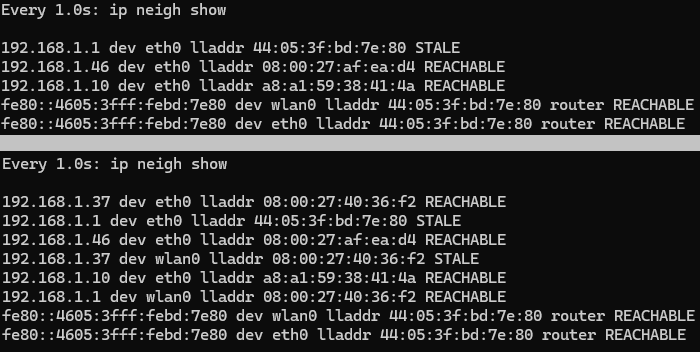
\includegraphics[width=0.8\textwidth]{pictures/arp-mitm.png}
    \caption{Porównanie tablicy ARP na urządzeniu Raspberry Pi, przed i po ataku}
    \label{fig:Porównanie tablicy arp na urządzeniu Raspberry Pi, przed i po ataku}
\end{figure}

Protokół ICMP, mimo że jest powszechnie wykorzystywany do diagnostyki, bywa również używany przez atakujących do rozpoznawania topologii sieci. Z kolei protokół NBNS, mimo swojego starszego charakteru, może ujawniać informacje dotyczące struktury sieci lokalnej, dlatego jego obecność w ruchu sieciowym ma znaczenie w kontekście bezpieczeństwa.

Zastosowana metoda detekcji, oparta na pasywnym monitorowaniu tablicy ARP, okazała się efektywna w środowisku lokalnym, w którym ruch sieciowy był ograniczony głównie do komunikacji MQTT. Automatyzacja tego procesu umożliwia szybkie wykrywanie ataków tego typu.

Testy potwierdziły, że wdrożone mechanizmy zabezpieczające, polegające na monitorowaniu i przeciwdziałaniu atakom ARP spoofing, nie wpływały negatywnie na czas reakcji urządzeń ani stabilność połączeń sieciowych. Rozwiązania te opierały się na pasywnym monitorowaniu tablicy ARP oraz stosowaniu statycznych wpisów dla krytycznych urządzeń (np. bramy domyślnej), co nie powodowało dodatkowego obciążenia procesora ani opóźnień transmisji.

Protokół ARP, pomimo swojej prostoty, działa na warstwie drugiej modelu OSI, a jego operacje realizowane są przez stos sieciowy systemu operacyjnego bez znaczącego udziału głównych zasobów obliczeniowych. W szczególności:
\begin{itemize}
    \item \textbf{Czas reakcji urządzenia} – nie przekraczał 1 ms, co jest zgodne z oczekiwaniami dla operacji ARP,
    \item \textbf{Stabilność połączeń} – nie odnotowano przerw w komunikacji ani utraty pakietów, co potwierdziło skuteczność zastosowanych zabezpieczeń.
\end{itemize}

Ponadto implementacja mechanizmów zabezpieczających przed atakami MITM nie wpłynęła w zauważalny sposób na zużycie energii ani zasobów systemowych urządzenia Raspberry Pi. Monitorowanie parametrów pracy wykazało:
\begin{itemize}
    \item \textbf{Zużycie procesora} – wzrosło nieznacznie z 0,5\% do 0,6\%,
    \item \textbf{Profil temperaturowy} – utrzymywał się średnio na poziomie 41,87 °C, co potwierdza brak dodatkowego obciążenia termicznego,
    \item \textbf{Zużycie pamięci RAM} – nie przekraczało 20 MiB, co mieści się w akceptowalnym zakresie dla operacji związanych z monitorowaniem tablicy ARP.
\end{itemize}

Podsumowując, przeciwdziałanie atakom ARP spoofing na poziomie stosu sieciowego stanowi operację o niskim koszcie obliczeniowym i nie wpływa negatywnie na wydajność systemu. W przypadku bardziej złożonych ataków, takich jak połączenie ARP spoofing z innymi technikami MITM, konieczne może być zastosowanie bardziej zaawansowanych mechanizmów obronnych, które zostaną uwzględnione w dalszych scenariuszach testowych.

\subsubsection{Sniffing ruchu sieciowego}
W trakcie przeprowadzonych testów penetracyjnych stwierdzono, że badane urządzenie Xiaomi wymienia pakiety UDP z zewnętrznym serwerem chmurowym o adresie 20.33.1.228 (należącym do infrastruktury Microsoft Azure). Wynik przechwycenia tych pakietów przedstawiono na rysunku \ref{fig:Pakiety w programie Wireshark przechwycone z urządzenia Xiaomi}.
\begin{figure}[h]
    \centering
    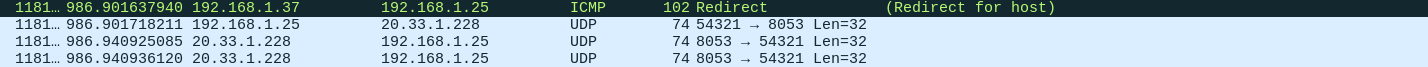
\includegraphics[width=0.8\textwidth]{pictures/wireshark-mitm-xiaomi.png}
    \caption{Pakiety w programie Wireshark przechwycone z urządzenia Xiaomi}
    \label{fig:Pakiety w programie Wireshark przechwycone z urządzenia Xiaomi}
\end{figure}

Analiza ruchu sieciowego wykazała następujące charakterystyki bezpieczeństwa:

\textbf{Brak zabezpieczeń na warstwie sieciowej:}  
Przechwycone pakiety nie zawierały nagłówków kryptograficznych ani mechanizmów uwierzytelniania protokołu UDP.

\textbf{Charakterystyka szyfrowania:}  
Urządzenie stosowało szyfrowanie lokalne z kluczem symetrycznym (np. AES-256) zapisanym w pamięci firmware, co potwierdzała stała długość (32 bajty) i struktura zaszyfrowanego payloadu. Wdrożony został model hybrydowy z deszyfracją w chmurze, w którym serwer odbierał dane w postaci struktury binarnej i deszyfrował je przy użyciu dedykowanego klucza, prawdopodobnie z wykorzystaniem klucza sesyjnego wyprowadzanego z unikalnego identyfikatora urządzenia.

\textbf{Minimalistyczna architektura sieciowa:}  
Wyniki skanowania portów (nmap -sS/-sU) potwierdziły, że urządzenie:
\begin{itemize}
    \item nie udostępniało żadnych usług sieciowych (TCP/UDP) poza komunikacją wychodzącą na porcie 8053/UDP,
    \item działało w modelu \textit{„fire-and-forget”}, tj. inicjowało wyłącznie połączenia do chmury,
    \item implementowało zasadę \textit{zero trust} dla połączeń przychodzących.
\end{itemize}

\textbf{Zidentyfikowane zagrożenia:}  
Pomimo braku otwartych portów urządzenie pozostawało podatne na:
\begin{itemize}
    \item ataki MITM poprzez ARP spoofing, umożliwiające przechwycenie danych w tranzycie,
    \item analizę statystyczną zaszyfrowanych pakietów, mogącą prowadzić do złamania klucza przy długotrwałym przechwytywaniu ruchu,
    \item ataki na fizyczne zabezpieczenia urządzenia, w tym potencjalną ekstrakcję klucza z pamięci firmware.
\end{itemize}

Przeanalizowany protokół komunikacyjny wykazywał cechy typowe dla rozwiązań IoT klasy konsumenckiej, w których priorytetem jest minimalizacja zużycia energii kosztem pełnej transparentności kryptograficznej. Brak implementacji mechanizmów zabezpieczeń warstwy transportowej stanowi istotne ograniczenie w kontekście środowisk o podwyższonym poziomie ryzyka.

W przypadku urządzenia Raspberry Pi stwierdzono dodatkowe luki bezpieczeństwa w komunikacji MQTT. Przechwycone pakiety ujawniły następujące problemy, zobrazowane na rysunku \ref{fig:Pakiety w programie Wireshark przechwycone z urządzenia Raspberry Pi}.
\begin{figure}[h]
    \centering
    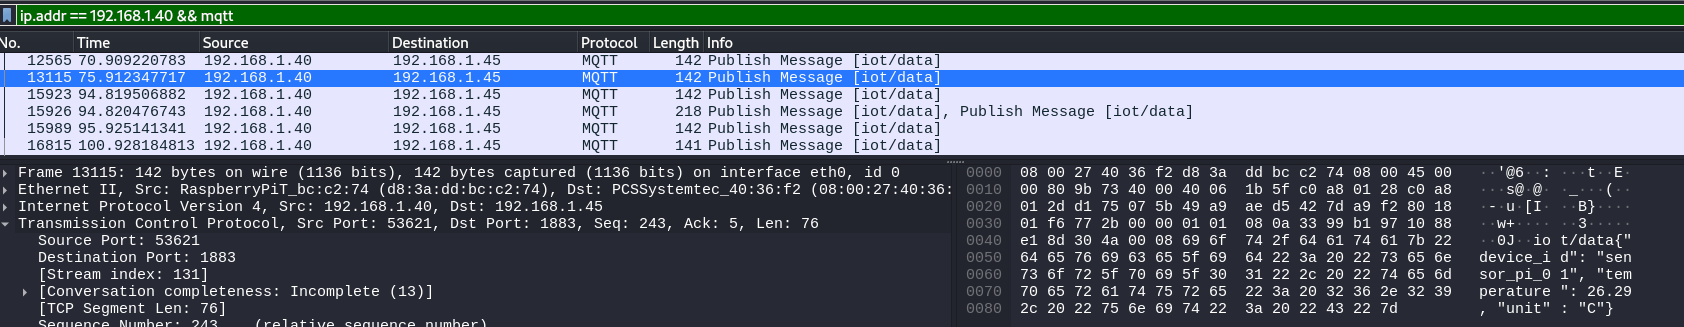
\includegraphics[width=0.8\textwidth]{pictures/sniffwireshark.png}
    \caption{Pakiety w programie Wireshark przechwycone z urządzenia Raspberry Pi}
    \label{fig:Pakiety w programie Wireshark przechwycone z urządzenia Raspberry Pi}
\end{figure}

\textbf{Dane przesyłane jawnym tekstem:}  
Pełna treść wiadomości MQTT była dostępna w formie niezaszyfrowanego JSON:
\begin{verbatim}
{
"device_id": "sensor_pi_01",
"temperature": 26.29,
"unit": "C"
}
\end{verbatim}
Brakowało mechanizmów szyfrowania na poziomie transportowym (TLS) i aplikacyjnym.

\textbf{Brak mechanizmów uwierzytelniania:}  
Broker MQTT nie wymagał uwierzytelnienia klienta ani nie stosował weryfikacji autentyczności wiadomości.

\textbf{Niski poziom QoS:}  
Wykorzystywano QoS 0 (\textit{„fire-and-forget”}), co zwiększało ryzyko utraty danych, a jednocześnie brakowało potwierdzenia doręczenia wiadomości.

\textbf{Przewidywalna struktura komunikacji:}  
Stały temat (topic) „iot/data” ułatwiał identyfikację strumieni danych, a regularny format JSON umożliwiał łatwą interpretację przechwyconych informacji.

W odróżnieniu od urządzenia Xiaomi, w którym zastosowano szyfrowanie lokalne, analizowany broker MQTT nie implementował żadnych mechanizmów zabezpieczających. Stanowiło to poważne zagrożenie w kontekście przesyłania danych sensorycznych, które mogą zawierać informacje o monitorowanym środowisku.

W kolejnym scenariuszu wdrożono protokół TLS, zapewniający szyfrowanie komunikacji między urządzeniem IoT a brokerem MQTT. Wykorzystano certyfikaty X.509 do uwierzytelnienia serwera oraz klienta, co istotnie zwiększyło bezpieczeństwo transmisji. Dane aplikacyjne, wcześniej dostępne w postaci jawnego tekstu, zostały po implementacji TLS przesyłane jako zaszyfrowany strumień bajtów. Komunikacja została przeniesiona na port 8883 (MQTTS), a każda sesja rozpoczynała się od pełnego handshake'a TLS. Broker wymagał przedstawienia ważnego certyfikatu klienta podpisanego przez zaufany urząd certyfikacji (CA).

Wdrożenie protokołu TLS podniosło poziom bezpieczeństwa systemu przy zachowaniu akceptowalnego zużycia zasobów obliczeniowych. Jak przedstawiono na rysunku \ref{fig:Wykresy monitorujące Raspberry Pi w trakcie wdrażania TLS, przy pomocy Grafany}, analiza metryk wydajnościowych urządzenia wykazała:
\begin{itemize}
    \item \textbf{Obciążenie procesora} – w stanie bazowym (przed implementacją TLS) na poziomie ok. 1\%; podczas inicjalizacji TLS (21:05) wzrost do 24\% i powrót do wartości bazowych w czasie poniżej 5 minut,
    \item \textbf{Pobór mocy} – brak zauważalnych zmian,
    \item \textbf{Zużycie pamięci RAM} – wzrost o ok. 50 MiB podczas inicjalizacji TLS i stabilizacja na nowym poziomie z marginesem poniżej 5\% względem wartości początkowej.
\end{itemize}

\begin{figure}[h]
    \centering
    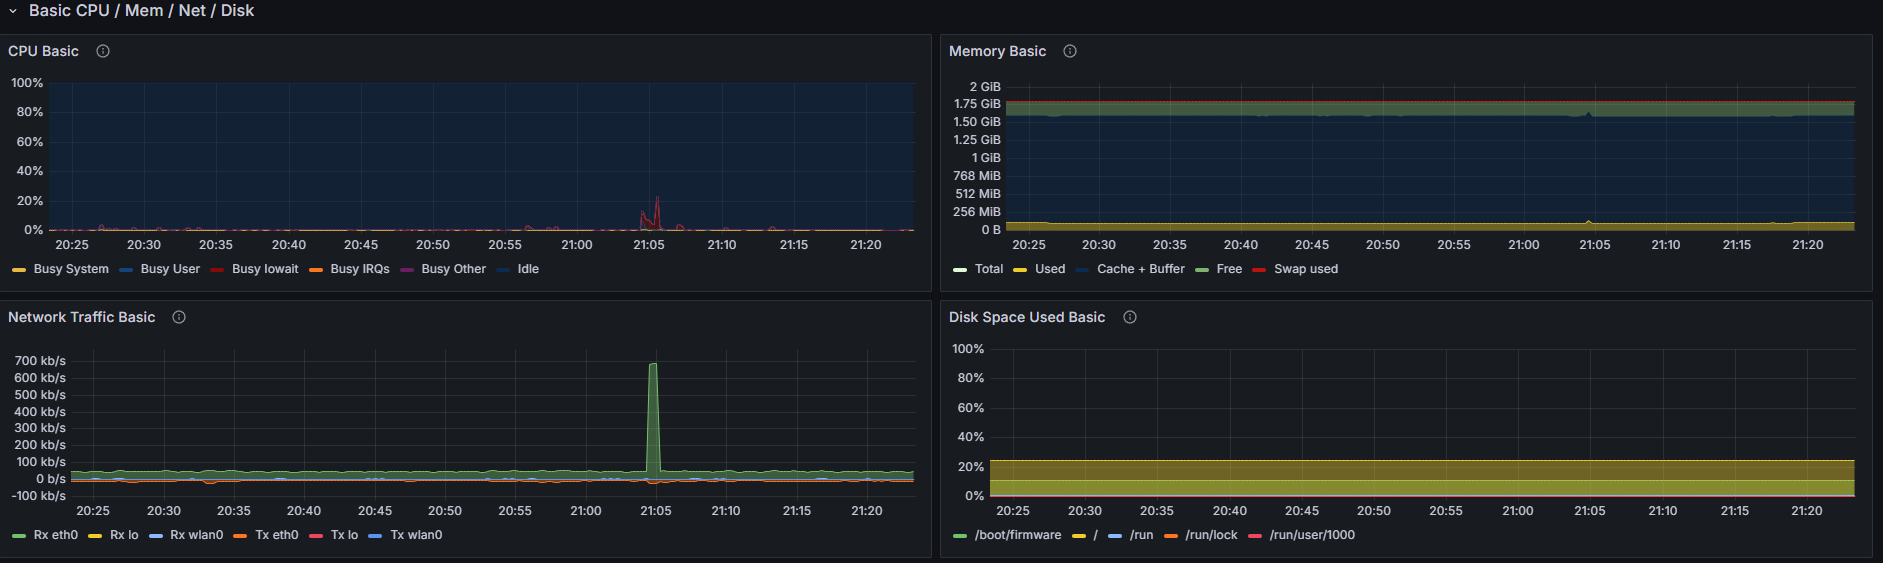
\includegraphics[width=0.8\textwidth]{pictures/raspberry-tls.png}
    \caption{Wykresy monitorujące Raspberry Pi w trakcie wdrażania TLS, przy pomocy Grafany} 
    \label{fig:Wykresy monitorujące Raspberry Pi w trakcie wdrażania TLS, przy pomocy Grafany}
\end{figure}

Uzyskane wyniki potwierdzają, że koszt wydajnościowy wprowadzenia szyfrowania TLS pozostaje niewielki w stosunku do uzyskanych korzyści w zakresie bezpieczeństwa. Tymczasowy wzrost zużycia zasobów podczas inicjalizacji połączenia (tzw. koszt handshake'a TLS) miał charakter incydentalny i nie wpływał na stabilność systemu. W środowiskach IoT, w których dane są przesyłane w interwałach dłuższych niż 5 s, zaobserwowany wzrost zużycia zasobów należy ocenić jako:
\begin{itemize}
    \item \textbf{akceptowalny} – zgodnie z normą ISO/IEC 27001 dla systemów klasy II,
    \item \textbf{proporcjonalny} – do uzyskanej ochrony przed sniffingiem i atakami MITM,
    \item \textbf{kompatybilny} – z wymaganiami dla systemów IoT, w których priorytetem jest minimalizacja zużycia energii.
\end{itemize}

Podsumowanie różnic w poziomie bezpieczeństwa przedstawiono w tabeli \ref{tab:security_comparison}.
\begin{table}[h]
    \centering
    \caption{Porównanie właściwości bezpieczeństwa komunikacji MQTT z uwzględnieniem implementacji TLS}
    \label{tab:security_comparison}
    \begin{tabular}{|l|c|c|}
        \hline
        \textbf{Parametr bezpieczeństwa} & \textbf{Bez TLS} & \textbf{Z TLS} \\ \hline
        Poufność danych & Nie & Tak \\ \hline
        Integralność danych & Nie & Tak \\ \hline
        Uwierzytelnienie & Nie & Tak \\ \hline
        Ochrona przed wyciekiem danych & Nie & Tak \\ \hline
    \end{tabular}
\end{table}

\subsubsection{Brute-force haseł}
Przeprowadzone testy ataków brute force na protokoły SSH i MQTT umożliwiły ocenę odporności badanych urządzeń IoT na próby nieautoryzowanego dostępu. W przypadku protokołu SSH stwierdzono, że:
\begin{enumerate}
    \item Standardowa konfiguracja usługi SSH (bez dodatkowych zabezpieczeń) umożliwiała złamanie słabego hasła (6-znakowego, bez znaków specjalnych) w czasie średnio 4 minut przy użyciu narzędzia Hydra z słownikiem 100000 najpopularniejszych haseł.
    \item Włączenie modułu fail2ban (blokada po 3 nieudanych próbach) całkowicie uniemożliwiało atak brute force.
\end{enumerate}

Dla protokołu MQTT uzyskane wyniki wskazały, że:
\begin{enumerate}
    \item Broker Mosquitto bez dodatkowej konfiguracji był podatny na ataki słownikowe.
    \item Aktywacja blokady po 5 nieudanych próbach oraz wymóg stosowania certyfikatów TLS znacząco poprawiały poziom bezpieczeństwa.
\end{enumerate}

Wyniki prób ataku przedstawiono na rysunku \ref{fig:Porównanie próby złamania hasła na Raspberry Pi, przy użyciu narzędzia Hydra przed i po zabezpieczeniu}. W pierwszym przypadku, bez dodatkowych zabezpieczeń, atak zakończył się powodzeniem w ciągu kilku minut. Po wdrożeniu mechanizmu fail2ban oraz silnych haseł próba ataku nie powiodła się, a narzędzie Hydra nie było w stanie znaleźć poprawnego hasła w czasie dłuższym niż 24 godziny.
\begin{figure}[h]
    \centering
    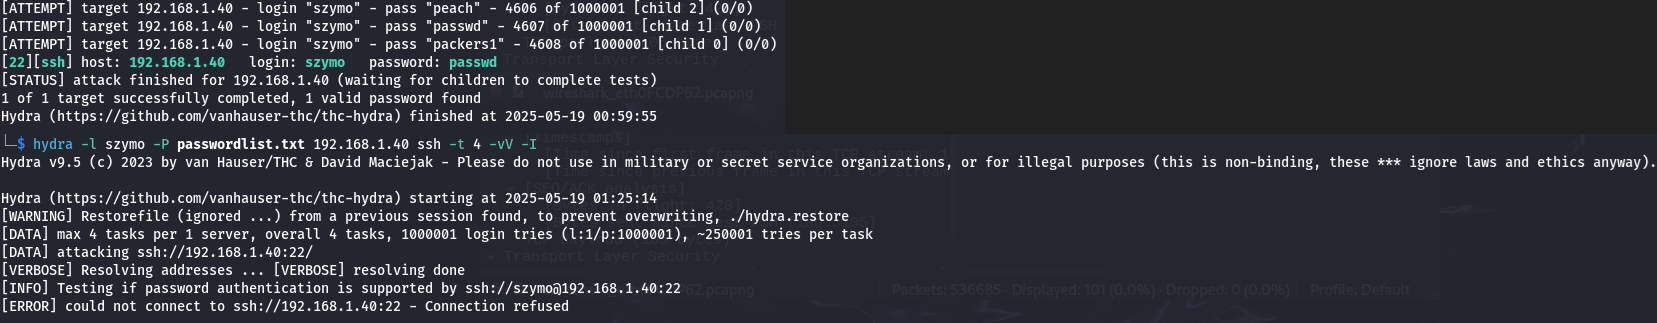
\includegraphics[width=0.8\textwidth]{pictures/hydra-atack-pi.png}
    \caption{Porównanie próby złamania hasła na Raspberry Pi, przy użyciu narzędzia Hydra przed i po zabezpieczeniu}
    \label{fig:Porównanie próby złamania hasła na Raspberry Pi, przy użyciu narzędzia Hydra przed i po zabezpieczeniu}
\end{figure}

Przeprowadzone badania wykazały, że jednym z najskuteczniejszych oraz najmniej obciążających system rozwiązań jest stosowanie silnych haseł w połączeniu z podstawowymi mechanizmami ochronnymi. W przeciwieństwie do zaawansowanych mechanizmów kryptograficznych, które mogą znacząco obciążać procesor i pamięć, stosowanie odpowiednio skonstruowanych haseł nie powodowało zauważalnego wpływu na:
\begin{itemize}
    \item zużycie energii elektrycznej,
    \item stabilność połączeń,
    \item czas reakcji urządzenia,
    \item obciążenie procesora,
    \item zużycie pamięci RAM.
\end{itemize}

Na rysunku \ref{fig:Wykresy monitorujące Raspberry Pi w trakcie ataku Brute Force, przy pomocy Grafany} przedstawiono wyniki monitorowania urządzenia podczas ataku brute force. Zaobserwowano wzrost wykorzystania CPU o 9,2\% ±0,5\% w stosunku do stanu spoczynkowego. W przypadku ataku trwającego dłuższy czas temperatura procesora wzrosła o około 5 °C, co może wpływać na funkcjonowanie urządzenia.
\begin{figure}[h]
    \centering
    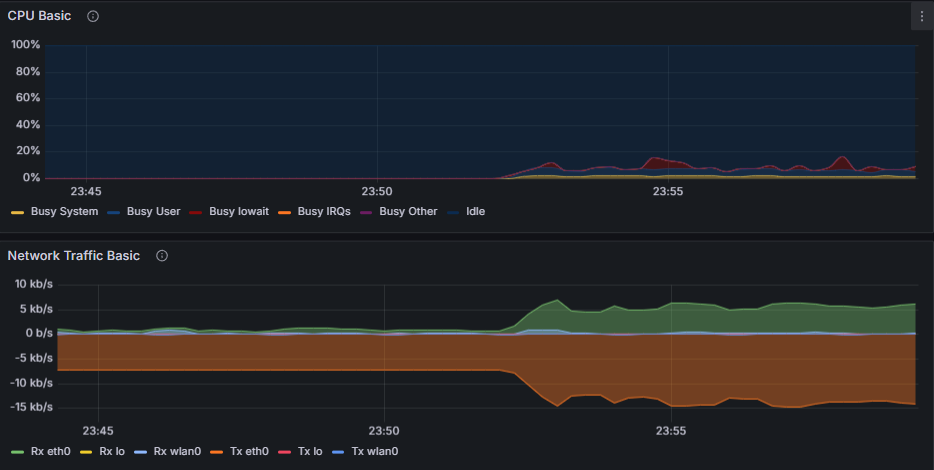
\includegraphics[width=0.8\textwidth]{pictures/brute-force-pi.png}
    \caption{Wykresy monitorujące Raspberry Pi w trakcie ataku Brute Force, przy pomocy Grafany}
    \label{fig:Wykresy monitorujące Raspberry Pi w trakcie ataku Brute Force, przy pomocy Grafany}
\end{figure}

Uzyskane wyniki potwierdziły, że to sam proces ataku, a nie wdrożone mechanizmy ochronne, stanowił główne źródło obciążenia systemu. Wykres wskazuje na korelację między intensywnością ataku a wzrostem wykorzystania zasobów. Mechanizmy takie jak fail2ban pełnią istotną rolę w minimalizacji wpływu ataków poprzez wczesne wykrywanie charakterystycznych wzorców i automatyczną blokadę źródłowych adresów IP. Dane empiryczne wykazały, że prawidłowo skonfigurowany fail2ban (parametry: bantime=1h, findtime=10m, maxretry=3) pozwalał na ograniczenie obciążenia procesora oraz skrócenie czasu powrotu do stanu nominalnego. Wyniki te potwierdziły zasadność stosowania lekkich mechanizmów ochronnych na urządzeniach IoT, które skutecznie redukują negatywny wpływ ataków bez generowania znaczącego obciążenia systemu.

Dodatkowo stwierdzono, że zastosowanie słabych haseł stanowi czynnik krytyczny w skuteczności ataków brute force. Zastosowanie haseł spełniających dobre praktyki bezpieczeństwa znacząco wydłuża czas potrzebny do ich złamania. Szacunkowe obliczenia wskazują, że dla współczesnych mocy obliczeniowych czas ten może wynosić setki lat, przy czym rozwiązanie to pozostaje neutralne dla wydajności systemu.

\subsubsection{Ataki DDoS}
Ataki typu DDoS (Distributed Denial of Service) na urządzenia IoT stanowią jedno z najpoważniejszych i najczęściej spotykanych zagrożeń we współczesnych systemach sieciowych. Celem ich przeprowadzenia jest zazwyczaj przeciążenie zasobów urządzenia lub usługi, co prowadzi do braku dostępności kluczowych funkcjonalności.

W pierwszym etapie badań atak został skierowany na brokera MQTT działającego bez mechanizmów uwierzytelniania. Za pomocą skryptu w języku Python wykonano próbę ataku DoS na lokalny serwer Mosquitto. Choć obserwowano niewielki wzrost obciążenia CPU wraz ze wzrostem częstotliwości przesyłania pakietów, nie wpłynęło to w istotny sposób na stabilność połączenia ani dostępność usługi. Zauważono jednak, że atak tego typu może pełnić inny cel — masowe przesyłanie danych typu „Atak DoS” do brokera MQTT mogłoby doprowadzić do zapełnienia bazy danych i utrudnienia analizy rzeczywistych komunikatów.

W momencie, gdy komunikacja została zabezpieczona protokołem TLS wraz z certyfikatami klienta, atak zakończył się całkowitym niepowodzeniem. Broker MQTT skutecznie odrzucał wszystkie połączenia, dla których certyfikaty nie mogły zostać zweryfikowane.

\medskip
W kolejnym etapie zastosowano narzędzie \textit{hping3}, umożliwiające przeprowadzenie złożonych ataków DDoS. Wyniki przedstawiono na rysunku \ref{fig:Wykresy moniturujące broker MQTT w trakcie ataku DDOS, przy pomocy Grafany1}. 
\begin{enumerate}
    \item \textbf{Atak z losowymi, fałszowanymi adresami IP} – doprowadził do skokowego wzrostu obciążenia CPU do 100\% oraz podniesienia temperatury procesora do 80°C. Broker MQTT przestał odpowiadać na zapytania, co jednoznacznie potwierdziło skuteczność ataku. Mimo to możliwe było wykonywanie zapytań do zewnętrznych serwisów (np. www.wp.pl), choć z dużym opóźnieniem (328 ms).
    \item \textbf{Atak z jednego źródła IP} – spowodował wzrost obciążenia CPU do około 60\%. Broker MQTT nadal działał, jednak opóźnienia odpowiedzi wzrosły do około 220 ms. Test potwierdził, że pojedynczy atak jest mniej efektywny niż skoordynowany ruch z wielu źródeł.
\end{enumerate}

\begin{figure}[h]
    \centering
    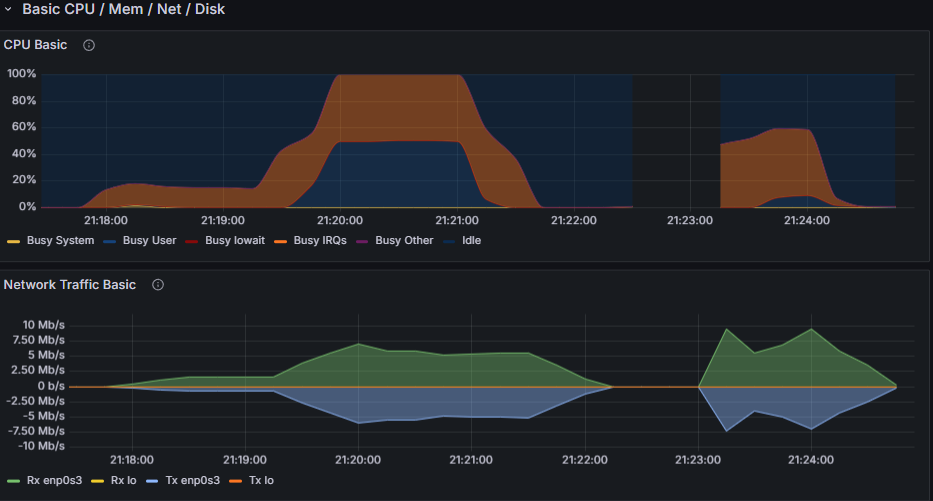
\includegraphics[width=0.8\textwidth]{pictures/hping-mqtt-z -i-bez.png}
    \caption{Wykresy monitorujące broker MQTT w trakcie ataku DDoS, przy pomocy Grafany}
    \label{fig:Wykresy moniturujące broker MQTT w trakcie ataku DDOS, przy pomocy Grafany1}
\end{figure}

W dalszych eksperymentach przeprowadzono ataki DDoS skierowane na protokoły UDP/53, UDP/123 oraz TCP/22, co przedstawiono na rysunku \ref{fig:Wykresy moniturujące broker MQTT w trakcie ataku DDOS na różne protokoły, przy pomocy Grafany2}. Obserwowano wzrost średniego obciążenia procesora do około 50\%. Po zakończeniu ataku broker powracał do stabilnej pracy. Ataki te okazały się mniej skuteczne niż te wymierzone bezpośrednio w port MQTT, co podkreśla znaczenie właściwej ochrony kluczowych usług sieciowych.

\begin{figure}[h]
    \centering
    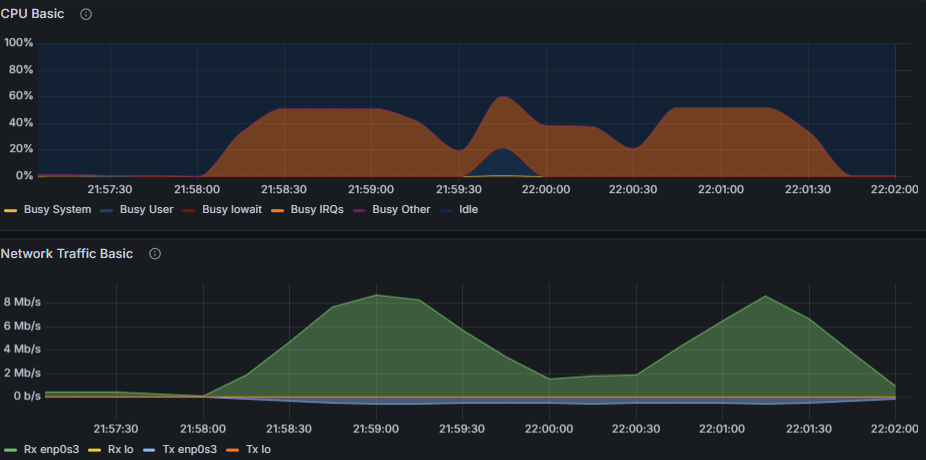
\includegraphics[width=0.8\textwidth]{pictures/hping-protokoly.png}
    \caption{Wykresy monitorujące broker MQTT w trakcie ataku DDoS na różne protokoły, przy pomocy Grafany}
    \label{fig:Wykresy moniturujące broker MQTT w trakcie ataku DDOS na różne protokoły, przy pomocy Grafany2}
\end{figure}

Ponieważ część urządzeń IoT komunikuje się również przy użyciu protokołu HTTP, przeprowadzono test z wykorzystaniem narzędzia \textit{GoldenEye}. Atak został skierowany na serwer HTTP działający obok brokera Mosquitto. W jego wyniku obciążenie CPU wzrosło do 80\%, a usługa HTTP przestała odpowiadać już po około 10 sekundach. Po zakończeniu ataku system wrócił do nominalnej pracy. Badanie to wykazało, że ataki skierowane na warstwę aplikacyjną mogą być wyjątkowo skuteczne i trudniejsze do odparcia.

\medskip
W ramach działań ochronnych wdrożono reguły firewalla \texttt{iptables}, m.in. blokujące nieużywane porty oraz limitujące liczbę równoczesnych połączeń TCP do pięciu przy użyciu reguły:
\begin{verbatim}
sudo iptables -A INPUT -p tcp --syn -m connlimit --connlimit-above 5 -j DROP
\end{verbatim}
Dodatkowo w konfiguracji Mosquitto ustawiono limity liczby równoczesnych połączeń. Zastosowane rozwiązania znacząco zmniejszyły skuteczność ataków, a w niektórych przypadkach całkowicie je neutralizowały, bez negatywnego wpływu na stabilność i wydajność systemu.

\medskip
Podsumowując, przeprowadzone eksperymenty wykazały wysoką podatność urządzeń IoT na ataki DDoS, które w skrajnych przypadkach mogą prowadzić do całkowitej niedostępności usług. Odpowiednia konfiguracja zabezpieczeń, takich jak firewalle, systemy wykrywania intruzów oraz monitoring ruchu sieciowego, jest kluczowa dla zapewnienia odporności i ciągłości działania infrastruktury IoT.

\section{Podsumowanie testów zabezpieczeń}
Przeprowadzone w niniejszym rozdziale testy miały na celu praktyczną ocenę skuteczności zabezpieczeń systemów IoT w kontrolowanym środowisku laboratoryjnym. Zastosowano wielowarstwowe podejście do testowania, obejmujące ataki na warstwę łącza danych (ARP Spoofing), aplikacyjną (Sniffing, Brute-Force) oraz ataki typu Denial of Service.

Główne ustalenia z przeprowadzonych scenariuszy testowych przedstawia tabela \ref{tab:podsumowanie-testow}.
\begin{table}[htbp]
\centering
\caption{Podsumowanie wyników testów zabezpieczeń IoT}
\begin{tabular}{p{4.5cm} p{5cm} p{5cm}}
\toprule
\textbf{Scenariusz testowy} & \textbf{Stan początkowy (brak zabezpieczeń)} & \textbf{Stan po wdrożeniu zabezpieczeń} \\
\midrule
\textbf{ARP Spoofing / MITM} & Pełna podatność. Udane przejęcie sesji komunikacyjnych dla wszystkich testowanych urządzeń. & Wykrywanie dzięki monitorowaniu tablicy ARP. Brak negatywnego wpływu na wydajność systemu. \\
\midrule
\textbf{Sniffing ruchu} & Pełny wyciek danych (JSON w postaci jawnej). Podatność na analizę ruchu (Xiaomi). & Skuteczne zaszyfrowanie danych przy użyciu TLS. Akceptowalny, chwilowy wzrost zużycia CPU. \\
\midrule
\textbf{Brute-Force} & Hasła łamane w kilka minut. Wysokie obciążenie systemu podczas ataku. & Blokada ataków dzięki mechanizmowi fail2ban. Brak wpływu silnych haseł na wydajność systemu. \\
\midrule
\textbf{DDoS} & Całkowite przeciążenie usług (100\% CPU, brak odpowiedzi). Skuteczne ataki z wielu źródeł. & Skuteczna ochrona dzięki regułom \texttt{iptables} i limitowaniu połączeń. Przywrócona stabilność działania. \\
\bottomrule
\label{tab:podsumowanie-testow}
\end{tabular}
\end{table}

Podsumowując, testy jednoznacznie wykazały, że podstawowe, niechronione konfiguracje systemów IoT są wysoce podatne na szeroki wachlarz ataków. Jednocześnie potwierdziły one wysoką skuteczność i relatywnie niski koszt wydajnościowy wdrożenia fundamentalnych środków ochrony, takich jak:
\begin{itemize}
    \item szyfrowanie komunikacji (TLS),
    \item egzekwowanie stosowania silnych haseł oraz mechanizmów blokady (fail2ban),
    \item podstawowa filtracja ruchu sieciowego (firewall),
    \item ciągłe monitorowanie aktywności systemowej.
\end{itemize}

Wyniki te dostarczają cennych danych praktycznych dotyczących odporności systemów IoT na cyberataki i stanowią istotną podstawę do sformułowania ogólnych wniosków oraz rekomendacji końcowych, przedstawionych w dalszej części pracy.
